\documentclass[xcolor=pdftex,dvipsnames,table,mathserif]{beamer}
\usetheme{default}
%\usetheme{Darmstadt}
%\usepackage{times}
%\usefonttheme{structurebold}

\usepackage[english]{babel}
%\usepackage[table]{xcolor}
\usepackage{pgf,pgfarrows,pgfnodes,pgfautomata,pgfheaps}
\usepackage{amsmath,amssymb,setspace}
\usepackage[latin1]{inputenc}
\usepackage[T1]{fontenc}
\usepackage{relsize}
\usepackage[absolute,overlay]{textpos} 
\newenvironment{reference}[2]{% 
  \begin{textblock*}{\textwidth}(#1,#2) 
      \footnotesize\it\bgroup\color{red!50!black}}{\egroup\end{textblock*}} 

\DeclareMathSizes{10}{10}{6}{6} 


\title [Dynamic Demand I]{Learning Models and Experience Goods}
\author{C.Conlon}
\institute{Grad IO }
\date{Fall 2016}
\setbeamerfont{equation}{size=\tiny}
\begin{document}

\begin{frame}
\titlepage
\end{frame}



\section*{Introduction}
%\begin{frame}{State Dependence}
%Think about a static model like BLP
%\begin{eqnarray*}
%u_{ijt} = \beta_i x_{jt} - \alpha_i p_{jt} + \xi_{jt} + \epsilon_{ijt}
%\end{eqnarray*}
%\begin{itemize}
%\item Suppose I have panel data on consumer $i$'s purchases and I observe that the consumer chooses different brands over time
%\item Why do you switch brands? 
%\begin{enumerate}
%\item New $\epsilon \rightarrow$ not helpful!
%\item Price responses $\rightarrow$ may wrongly attribute all effects to price.
%\item $\xi_{jt}$ not correlated across individuals but may include things like advertising, etc.
%\end{enumerate}
%\item Challenge is explaining both \alert{persistence} and \alert{switching} behavior.
%\end{itemize}
%\end{frame} 



\begin{frame}{Uncertainty and Learning}
\begin{itemize}
\item We have already looked at models with forward looking consumers
\item Consumers faced uncertainty about the price, but understood the characteristics and the utility received from the good up to the IID $\epsilon$.
\item In many cases, consumers do not fully understand their preferences over goods until they sample the goods themselves.
\item Changes to brands, introduction of new brands, price cuts, coupons, or advertising may induce consumers to resample.
\item We would like to incorporate \alert{persistence} in brand choice but also \alert{experiential learning}
\end{itemize}
\end{frame} 


 
\begin{frame}{Uncertainty and Learning}
We examine three papers dealing with uncertainty and learning:
\begin{itemize}
\item Ackerberg (2001) looks at whether advertising lets consumers learn about new brands and distinguishes between informative and prestige effects
\item Erdem and Keane (1996) extends models of brand choice to allow for Bayesian learning about experience goods
\item Crawford and Shum (2005) look at how doctor's learn about patient's types as well as drug efficacy in a model of experiential learning.
\end{itemize}
\end{frame}

\section*{Ackerberg}
\begin{frame}{Ackerberg 2001: Advertising and Yoplait 150}
\begin{itemize}
\item \textbf{Informative} about product existence and search characteristics. Stigler (1961), Butters (1977), Grossman Shapiro (1984) should not affect behavior of experienced users.
\item \textbf{Signalling} Nelson (1974), Kihlstrom and Riordan (1984), Milgrom and Roberts (1986).
\begin{enumerate}
\item If consumer perfectly learns about brand's experience characteristics after consumption $\rightarrow$ does not affect behavior of experienced users
\item If consumer continues to learn about  experience characteristics after consumption $\rightarrow$ should be decreasing in number of consumption experiences.
\end{enumerate}
\item \textbf{Prestige} Becker or Becker and Murphy (1993) does not depend on whether or not consumers have experienced the good but enters utility.
\end{itemize}
\end{frame}

\begin{frame}{Ackerberg 2001: Advertising and Yoplait 150}
\begin{itemize}
\item Ackerberg exploits panel data following advertising and grocery purchases over time.
\item Hypothesis is that \alert{informative} advertising has a larger effect on consumers with no brand experience.
\item \alert{Prestige} affects all consumers equally independent of experience.
\item Looks at a new product introduction to get around \alert{initial conditions problem}
\end{itemize}
\end{frame}

\begin{frame}{Ackerberg 2001: Data}
\begin{itemize}
\item AC Neilsen \textit{Scanner Data} matched upw ith TV meters
\item 1986-1989 covers 2000 households and 80\% of area drugstores and supermarkets.
\item Two cities: Sioux Falls, SD \alert{(SF)} and Springfield, MO \alert{(SP)}
\item He chooses yogurt because it is not easily storable (Hendel Nevo 2007).
\item Introduction of \alert{Yoplait 150} by the \#2 manufacturer
\item Heavily advertised, first low-fat, low-calorie yogurt by Yoplait!
\end{itemize}
\end{frame}

\begin{frame}{Table 1: Descriptive Statistics}
\begin{figure}[htbp]
\begin{center}
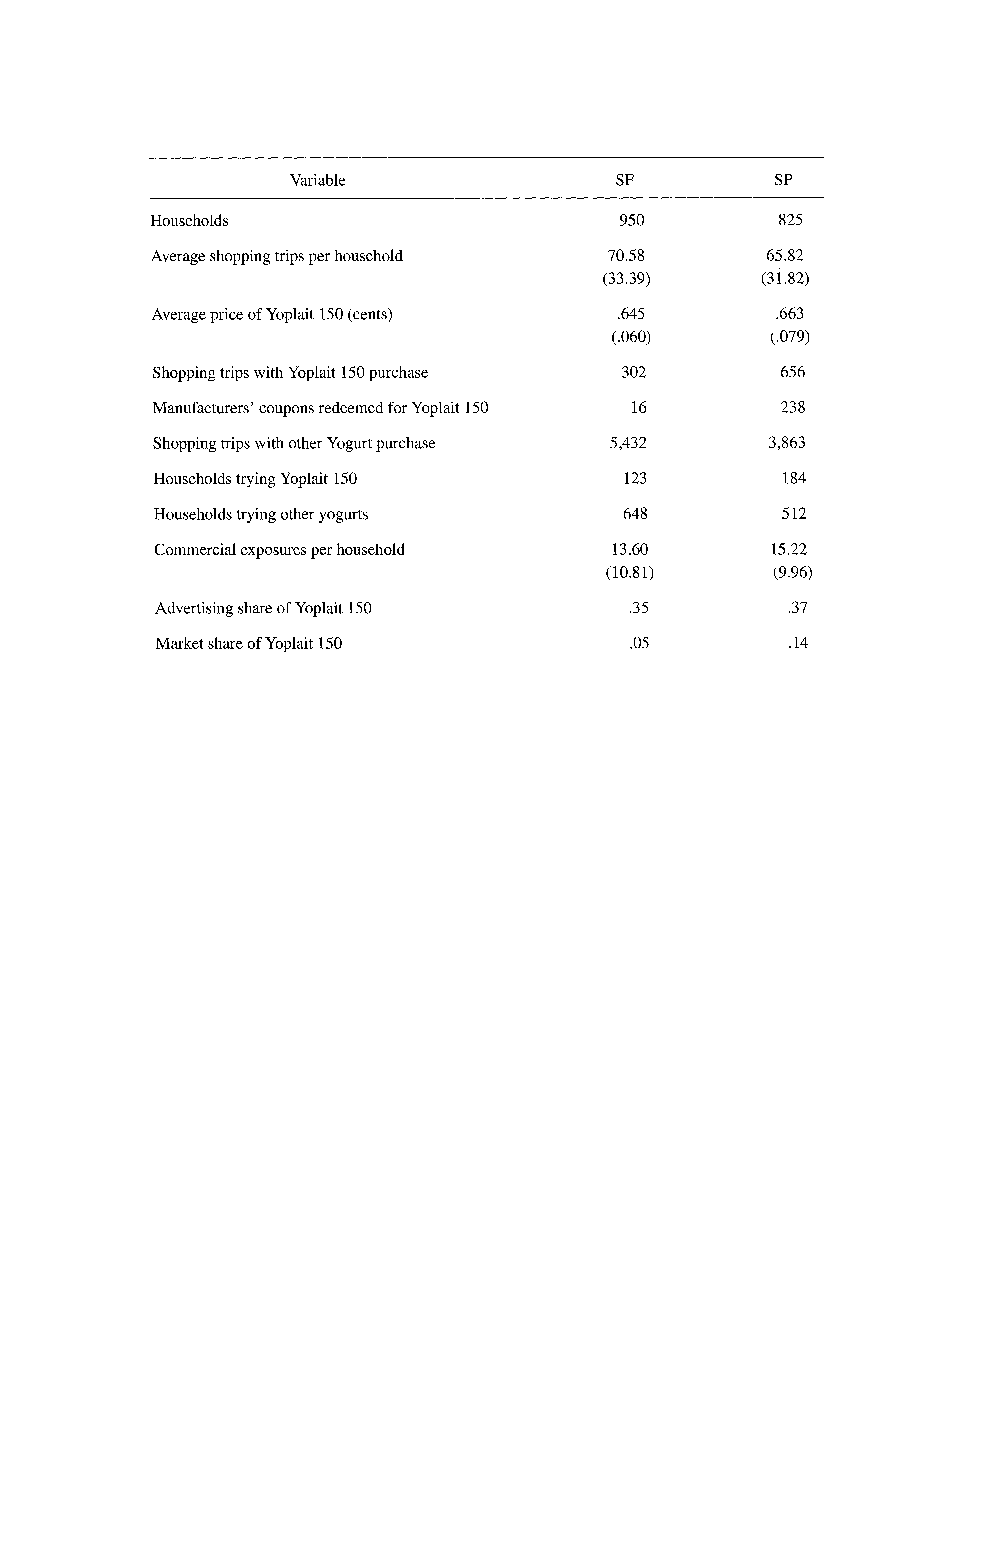
\includegraphics[width=8.5cm]{resources/acker1.pdf}
\label{default}
\end{center}
\end{figure}
\end{frame}

\begin{frame}{Table 2: Descriptive Correlations}
\begin{figure}[htbp]
\begin{center}
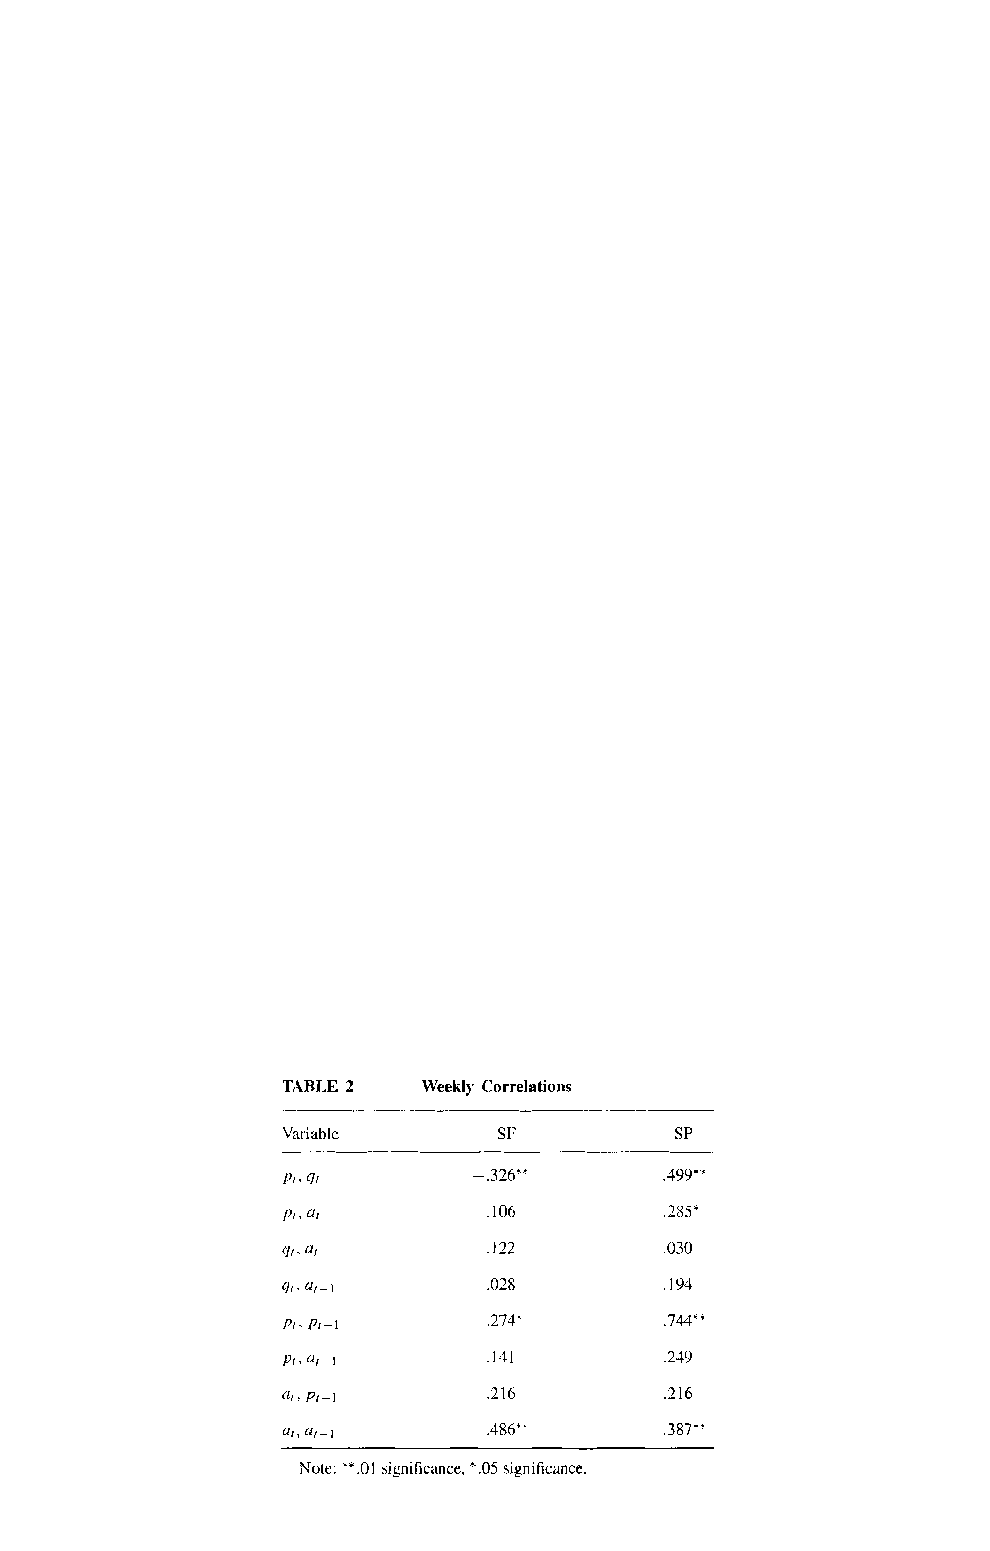
\includegraphics[width=9.5cm]{resources/acker2.pdf}
\label{default}
\end{center}
\end{figure}
\end{frame}

\begin{frame}{Table 3: Reduced Form Results}
\begin{figure}[htbp]
\begin{center}
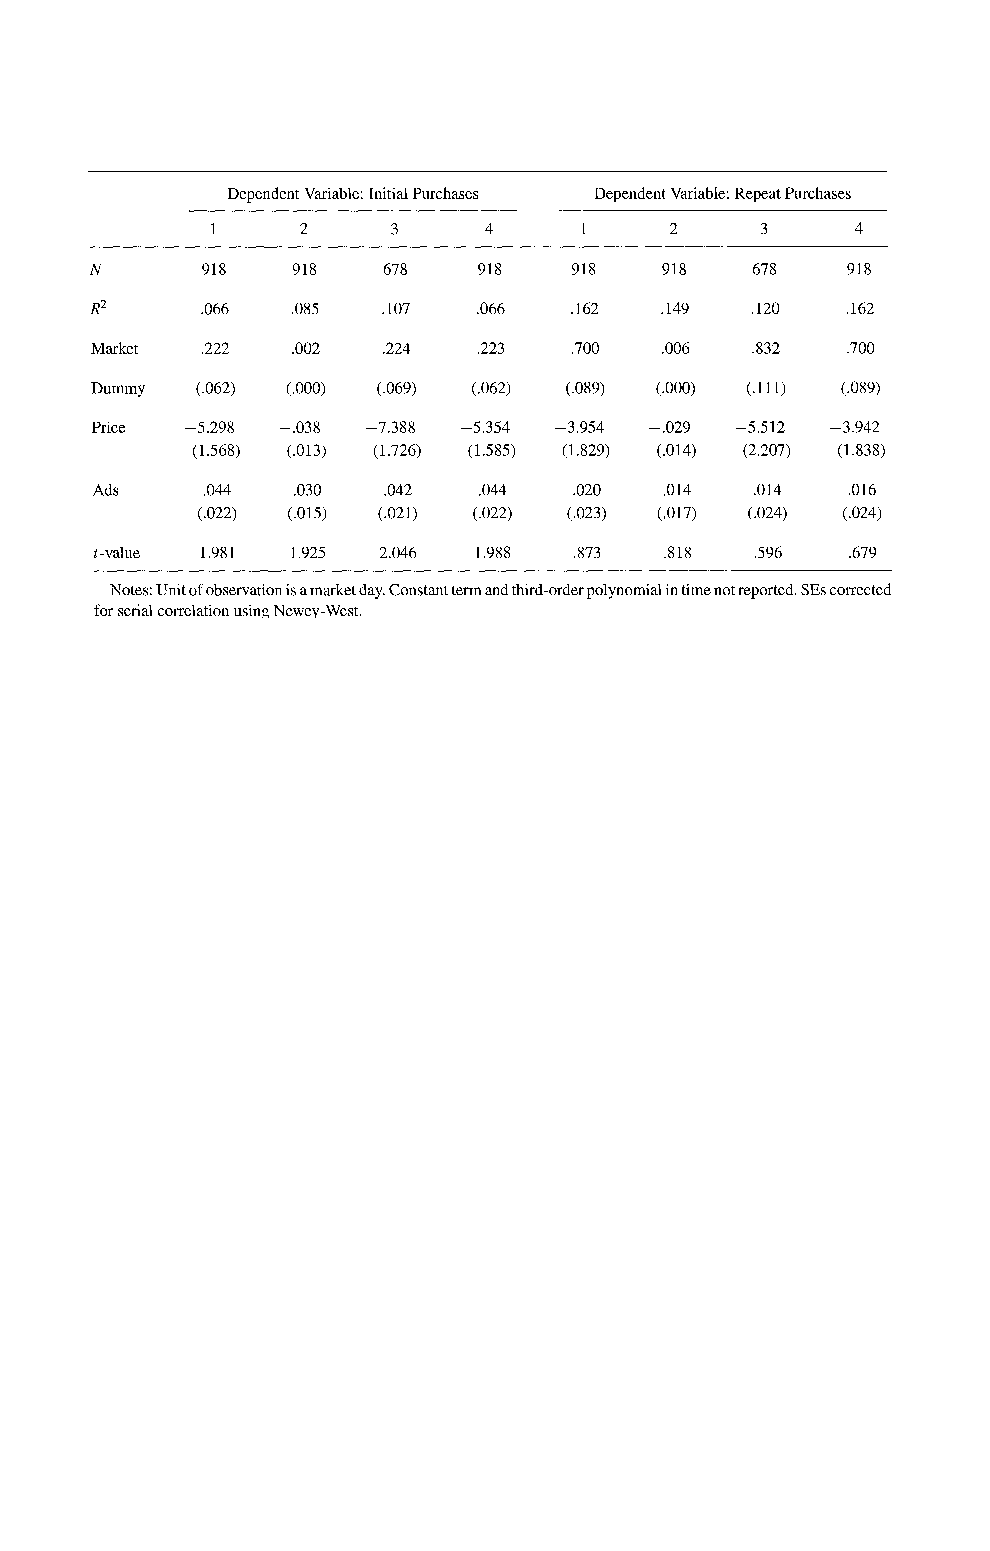
\includegraphics[width=9.5cm]{resources/acker3.pdf}
\label{default}
\end{center}
\end{figure}
\end{frame}



\begin{frame}{Model}
Reduced form for discrete choice that consumer $i$ purchases Yoplait 150 on trip $t$
\begin{eqnarray*}
c_{it} = \begin{cases}
       1 & \mbox{ IFF } \alpha_i + X_{it} \beta_1 - \gamma p_{it} + \epsilon_{1it} > Z_{it} \beta_2 + \epsilon_{2it}\\
       0 & \mbox{ o.w. } 
        \end{cases}
\end{eqnarray*}
\begin{itemize}
\item First term may \alert{proxy} for static utility or choice specific value function of YP150 purchase
\item Second term represents utility of outside option
\item $\alpha_i$ is a random effect (persistent heterogeneity) for YP150.
\item $X_{it}$ contains \alert{advertising}, household and consumer characteristics, and functions of previous purchases of YP150, coupon, time trend.
\item $Z_{it}$ contains an index of other competitors' prices
\end{itemize}
\end{frame}

\begin{frame}{Likelihood}
\begin{eqnarray*}
L_i(\theta) &=& Pr[c_{i1},\ldots,c_{iT_i} | W_i^t, Z_i^t, p_i^t; \theta] \\
&=& \int Pr[c_{i1},\ldots,c_{iT_i} | W_i^t, Z_i^t, p_i^t; a_i;  \theta] f(d \alpha_i | \theta)\\
&=& \int \prod_{t=1}^{T_i} Pr[c_{it}|  X_{it}(c_{i}^{t-1}), Z_{it}, p_{it}; a_i;  \theta] f(d \alpha_i | \theta)
\end{eqnarray*}
\begin{itemize}
\item $c_{i}^{t-1}$ is your entire purchase history
\item $W_{i}^t$ is the subset of explanatory variables $X_{it}$ that are completely exogenous
\item Choice probabilities determined by $\epsilon$ IID logit.
\end{itemize}
\end{frame}

\begin{frame}{Table 4: Structural Parameters}
\begin{figure}[htbp]
\begin{center}
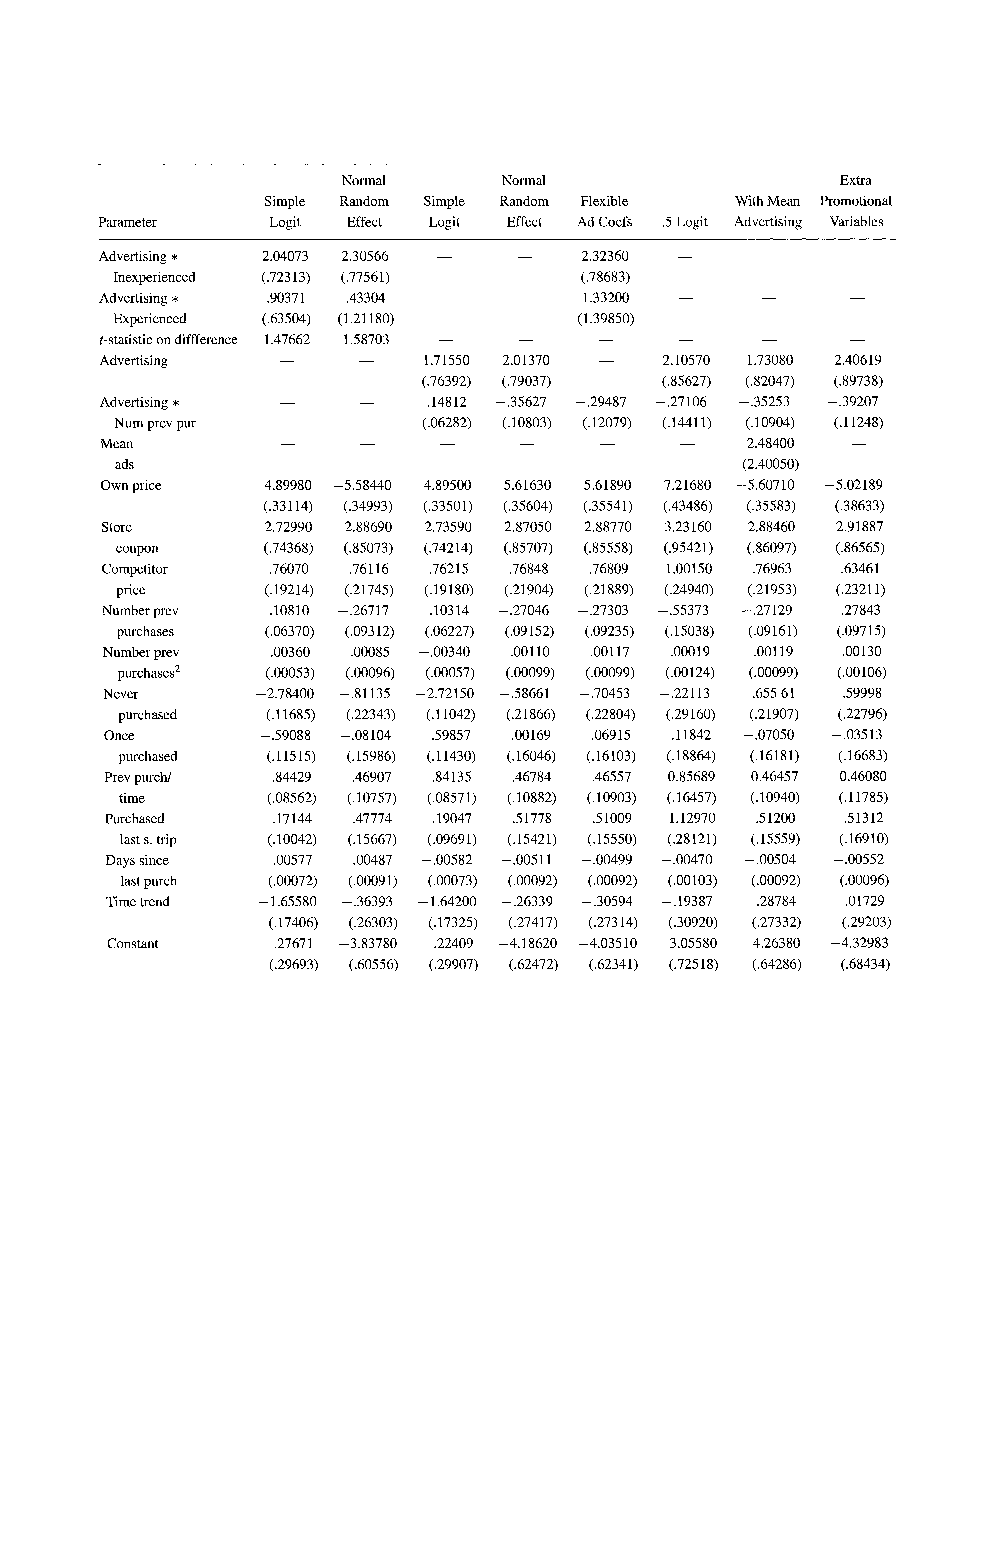
\includegraphics[width=8.5cm]{resources/acker4.pdf}
\label{default}
\end{center}
\end{figure}
\end{frame}

\begin{frame}{Discussion}
\begin{itemize}
\item Adv*Exp \alert{insignificant} image and prestige
\item Adv*Inexp - Adv*Exp: \alert{significant} informative
\item 30-sec commercial each week is like 10 cent price decrease
\item Adv*NPurch: decreasing returns to advertising
\end{itemize}
\end{frame}

\section*{Erdem and Keane}

\begin{frame}{Erdem Keane}
\begin{itemize}
\item Many markets are characterized by lots of new brands, price changes, and brand repositioning (especially CPG).
\item Nevo (2001) has hundreds of cereal brands enter and exit, similar in laundry detergent
\item Consumers may spend time experimenting with different brands to learn about them.
\item After learning takes place there may be state dependence until new brands are introduced or price cuts.
\end{itemize}
\end{frame} 

\begin{frame}{Guardini Little (Pre-Dynamics)}
\begin{eqnarray*}
E[U_{ij} | I_i(t) ] = a_j -w_P P_j + w_E \sum_{s=0}^t D_{1ijs}  + w_{Ad} \sum_{s=t_0}^t D_{2ijs}
\end{eqnarray*}
\begin{itemize}
\item $a_j$ mean brand taste for $j$
\item $D_{1ijt}$: dummy of whether consumer purchases brand $j$ or not
\item $D_{2ijt}$: dummy of whether consumers receives an advertising signal of brand $j$ or not
\item $w$ are utility weights (Lancaster 1966)
\end{itemize}
\end{frame} 


\begin{frame}{Erdem Keane: Decision-making Under Uncertainty}
\begin{itemize}
\item Consumer $i$ chooses among $J$ products in $T$ periods of time.
\item $d_{ij}(t)=1$ if consumer chooses $j$ (0 o.w.)
\item Includes an \textit{other brand} option
\item $E[U_{ij}(t) | I_i(t)]$ is current period expected utility conditional on information set $I_i(t)$.
\end{itemize}
Consumers maximize a discounted stream of expected utilities producing the Bellman:
\begin{eqnarray*}
V_{ij}(I_i(t),t) &=& E[U_{ij}(t) | I_i(t)] + \beta E[V(I(t+1),t+1) | I(t)] \\
V_i(I(t),t) &=& \max_j V_j(I_j(t),t)
\end{eqnarray*}
\end{frame}


\begin{frame}{Attribute Uncertainty}
\begin{itemize}
\item $A_{ijt} = A_j + \xi_{ijt} $ with i.i.d. mean zero shock $\xi_{ijt}$
\item Consumers don't immediately learn about attribute levels, instead:
\item $A_{E_{ijt}} = A_{ijt} + \eta_{ijt}$ with mean zero i.i.d disturbance $\eta_{ijt}$.
\item $A_{E_{ijt}} = A_{j} + \delta_{ijt}$ where $\delta_{ijt} = \xi_{ijt} + \eta_{ijt}$.
\item Empirically can't differentiate between private value $\xi_{ijt}$ and experience shock $\eta_{ijt}$.
\end{itemize}
\end{frame}

\begin{frame}{Consumer Expected Utility}
Additive Compensatory Multiattribute utility model. (Fishbein 1967) (Lancaster 1966)
\begin{eqnarray*}
U_{ijt} &=& -w_p P_{ijt} + w_A A_{E_{ijt}} - w_A r A_{E_{ijt}}^2 + e_{ijt}\\
E[U_{ijt} | I_i(t)] &=& -w_j P_{ijt} + w_A E[A_{E_{ijt}} | I(t)] - w_A r E [A_{E_{ijt}} | I_i(t)]^2\\
&&-w_A r E[A_{E_{ijt}} - E[A_{E_{ijt}}^2 | I_i(t)]]^2 + e_{ijt}
\end{eqnarray*}
Where $r$ is your risk parameter:  $r > 0$ risk averse
\begin{eqnarray*}
EU_{i0t}  &=& \Phi_{O} + \Phi_{Ot} + \epsilon_{i0t}\\
EU_{iNPt}  &=& \Phi_{NP} + \Phi_{NPt} + \epsilon_{iNPt}
\end{eqnarray*}
For outside good or other good.
\end{frame}

\begin{frame}{Bayesian Learning}
With no experience initial variability $\delta_{ijt}$, and advertising signal $S_{ijt}$
\begin{eqnarray*}
\delta_{ijt} \sim N(0,\sigma_{\delta}^2),  \quad& A_j \sim N(A,\sigma_A^2(0))\\
S_{ijt} = A_j + \zeta_{ijt}, \quad &\zeta_{ijt} \sim N(0,\sigma_{\zeta}^2)
\end{eqnarray*}
Consumers update:
\begin{eqnarray*}
E[A_{E_{ij,t+1}} | I_i(t)] &=&  E[A_{E_{ijt}} | I_i(t-1)] \\
 &-& D_{1ijt} \beta_{1ij}(t) [A_{E_{ijt}} - E[A_{E_{ijt}} | I_i(t-1)] ] \\
 &+&D_{2ijt} \beta_{2ij}(t) [S_{E_{ijt}} - E[S_{E_{ijt}} | I_i(t-1)] ] \\
\end{eqnarray*}
\end{frame}

\begin{frame}{Bayesian Learning}
\begin{itemize}
\item $D_{1ijt}$: dummy of whether consumer purchases brand $j$ or not
\item $D_{2ijt}$: dummy of whether consumers receives an advertising signal of brand $j$ or not
\item Kalman Filter Update
\begin{eqnarray*}
\beta_{1ijt} = \frac{ \sigma_{vij}^2(t)} { \sigma_{vij}^2(t) + \sigma_{\delta}^2}, &\quad& 
\beta_{2ijt} = \frac{ \sigma_{vij}^2(t)} { \sigma_{vij}^2(t) + \sigma_{\zeta}^2}\\
v_{ij} &=& E[A_{ij} | I_{ij}(t)] - A_j
\end{eqnarray*} 
\item And
\begin{eqnarray*}
A_{j} &=& E[A_j | I_{ij}(t)] + v_{ij}(t)\\
A_{E_{ijt}} &=& A_j + \delta_{ijt} , \quad S_{ijt} = A_j + \zeta_{ijt}
\end{eqnarray*} 
\end{itemize}
\end{frame}

\begin{frame}{Bayesian Learning}
\begin{eqnarray*}
v_{ijt}(t) &=& v_{ij}(t-1) + D_{1ijt} \beta_{1ij}(t)[-v_{ij}(t-1) + \delta_{ijt}]  \\
&+& D_{2ijt} \beta_{2ij}(t)[-v_{ij}(t-1) + \zeta_{jt}]\\
\sigma_{vij}^2(t) &=& \frac{1}{\frac{1}{\sigma_v^2(0)} + \frac{\sum_{s=0}^t D_{1ijs}}{\sigma_{\delta}^2} + \frac{\sum_{s=0}^t D_{2ijs}}{\sigma_{\zeta}^2}}
\end{eqnarray*}
And expected utilities:
\begin{eqnarray*}
E[U_{ij} | I_i(t)] &=& w_A A_j - w_A r A_j^2 -w_A r \sigma_{\delta}^2 -w_P P_{ij} \\
&-& -w_A r \sigma_{vij}^2(t) - w_A r v_{ij}(t)^2  - w_A v_{ij}(t) - 2w_A r A_j v_{ij} (t) \\ &+& e_{ijt}\\
E[V_{ij} | I_i(t)] &=& E[U_{ij} | I_i(t)] + \beta E[V_{ij} | I_i(t+1) | d_{ijt} =1, I_i(t)]
\end{eqnarray*}
\end{frame}


\begin{frame}{Choice Probabilities}
For the Static and Dynamic case:
\begin{eqnarray*}
P^s_i(I(t),t) = \int \frac{\exp [E [U_{ij} | I_i(t)] ] } {\sum_k \exp [E [U_{ik} | I_i(t)] ] } f(v) dv\\
P^d_i(I(t),t) = \int \frac{\exp [E [V_{ij} | I_i(t)] ] } {\sum_k \exp [E [V_{ik} | I_i(t)] ] } f(v) dv
\end{eqnarray*}
\begin{itemize}
\item Static model allows choices to depend on 
\alert{current knowledge of attribute}
\item Static model does not incorporate \alert{value of learning for future consumption}
\item Logit choice probabilities but with time varying random coefficients
\item Everything about learning in is in the distribution of $v$
\end{itemize}
\end{frame}


\begin{frame}{Data}
\begin{itemize}
\item Laundry detergent scanner data from 1986-1988.
\item 3000 HH's w/ 20 purchases (7 liquid)
\item Lots of advertising
\item Only liquids (80\% of market)
\item Many new brands
\item  TVs measures ad exposure
\begin{itemize}
\item Percentage of weeks household saw brand $j$'s ad.
\item Saw at least one ad during that week
\end{itemize}
\end{itemize}
\end{frame}


\begin{frame}{Table 2: Static Model No Learning} 
\begin{figure}[htbp]
\begin{center}
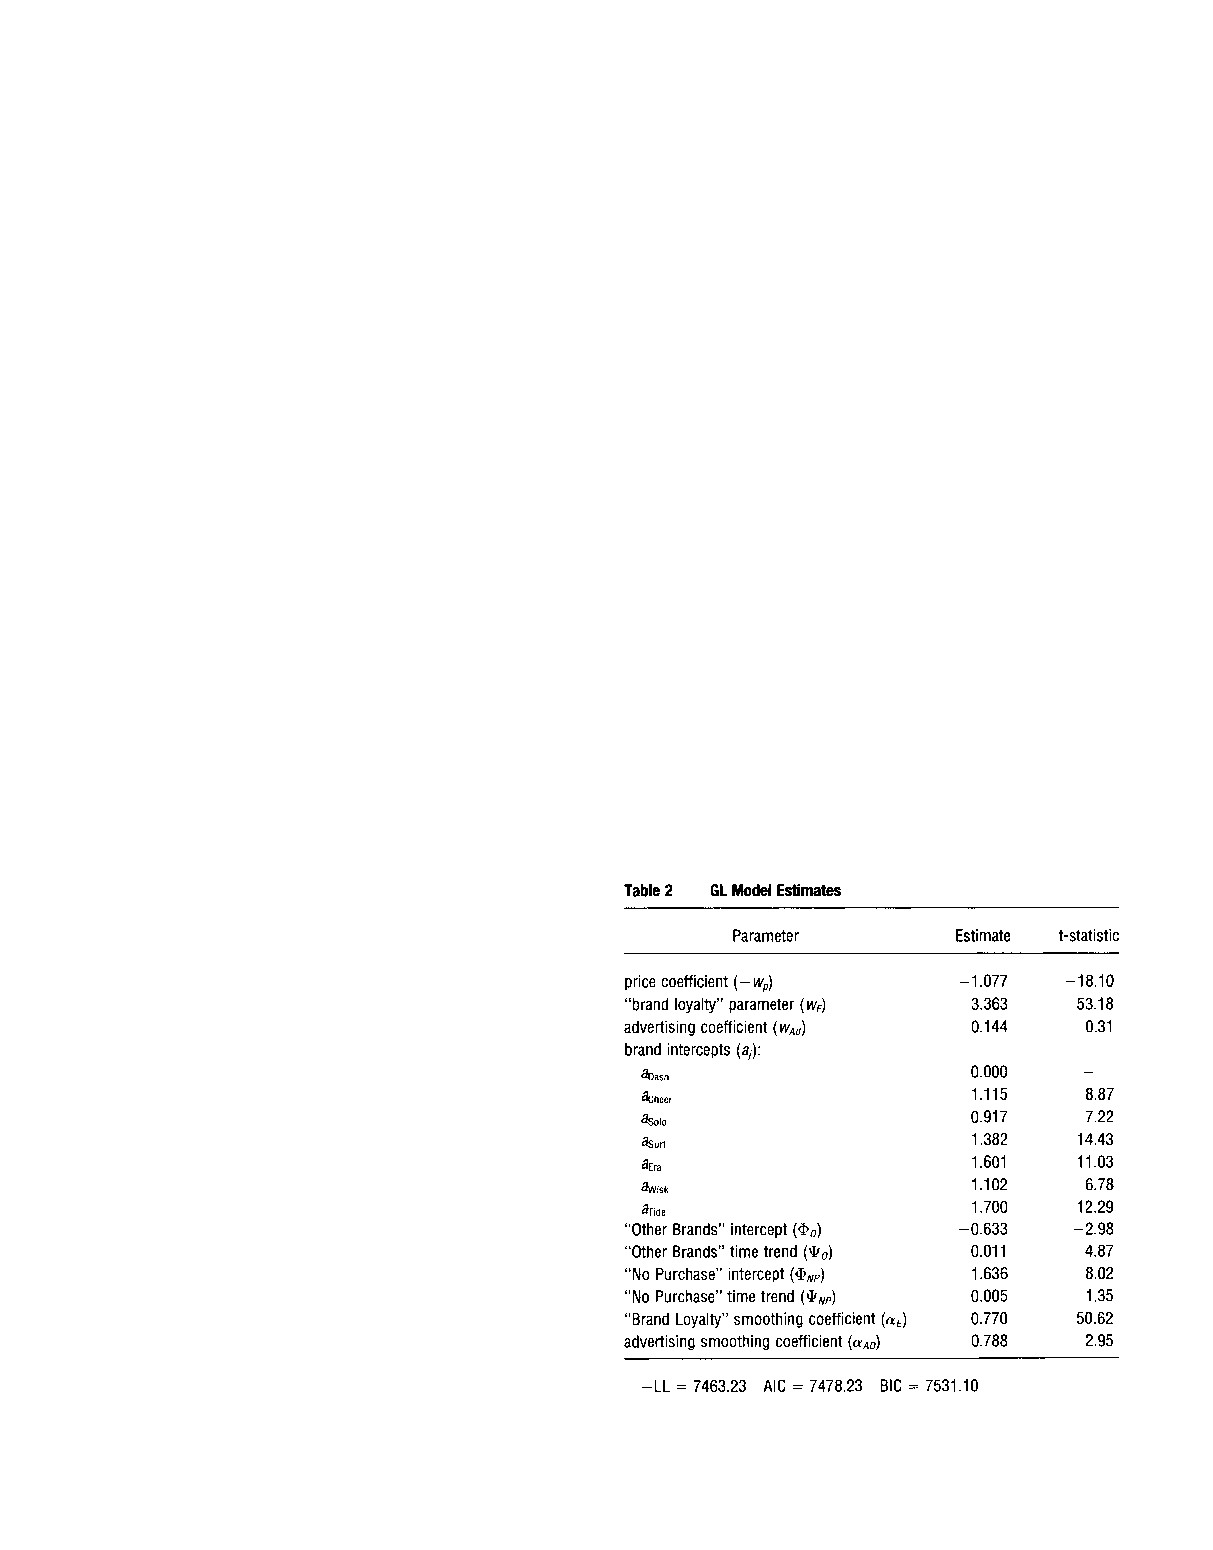
\includegraphics{resources/ek1.pdf}
\label{default}
\end{center}
\end{figure}
\end{frame}

\begin{frame}{Table 3: Dynamic Model}
\begin{figure}[htbp]
\begin{center}
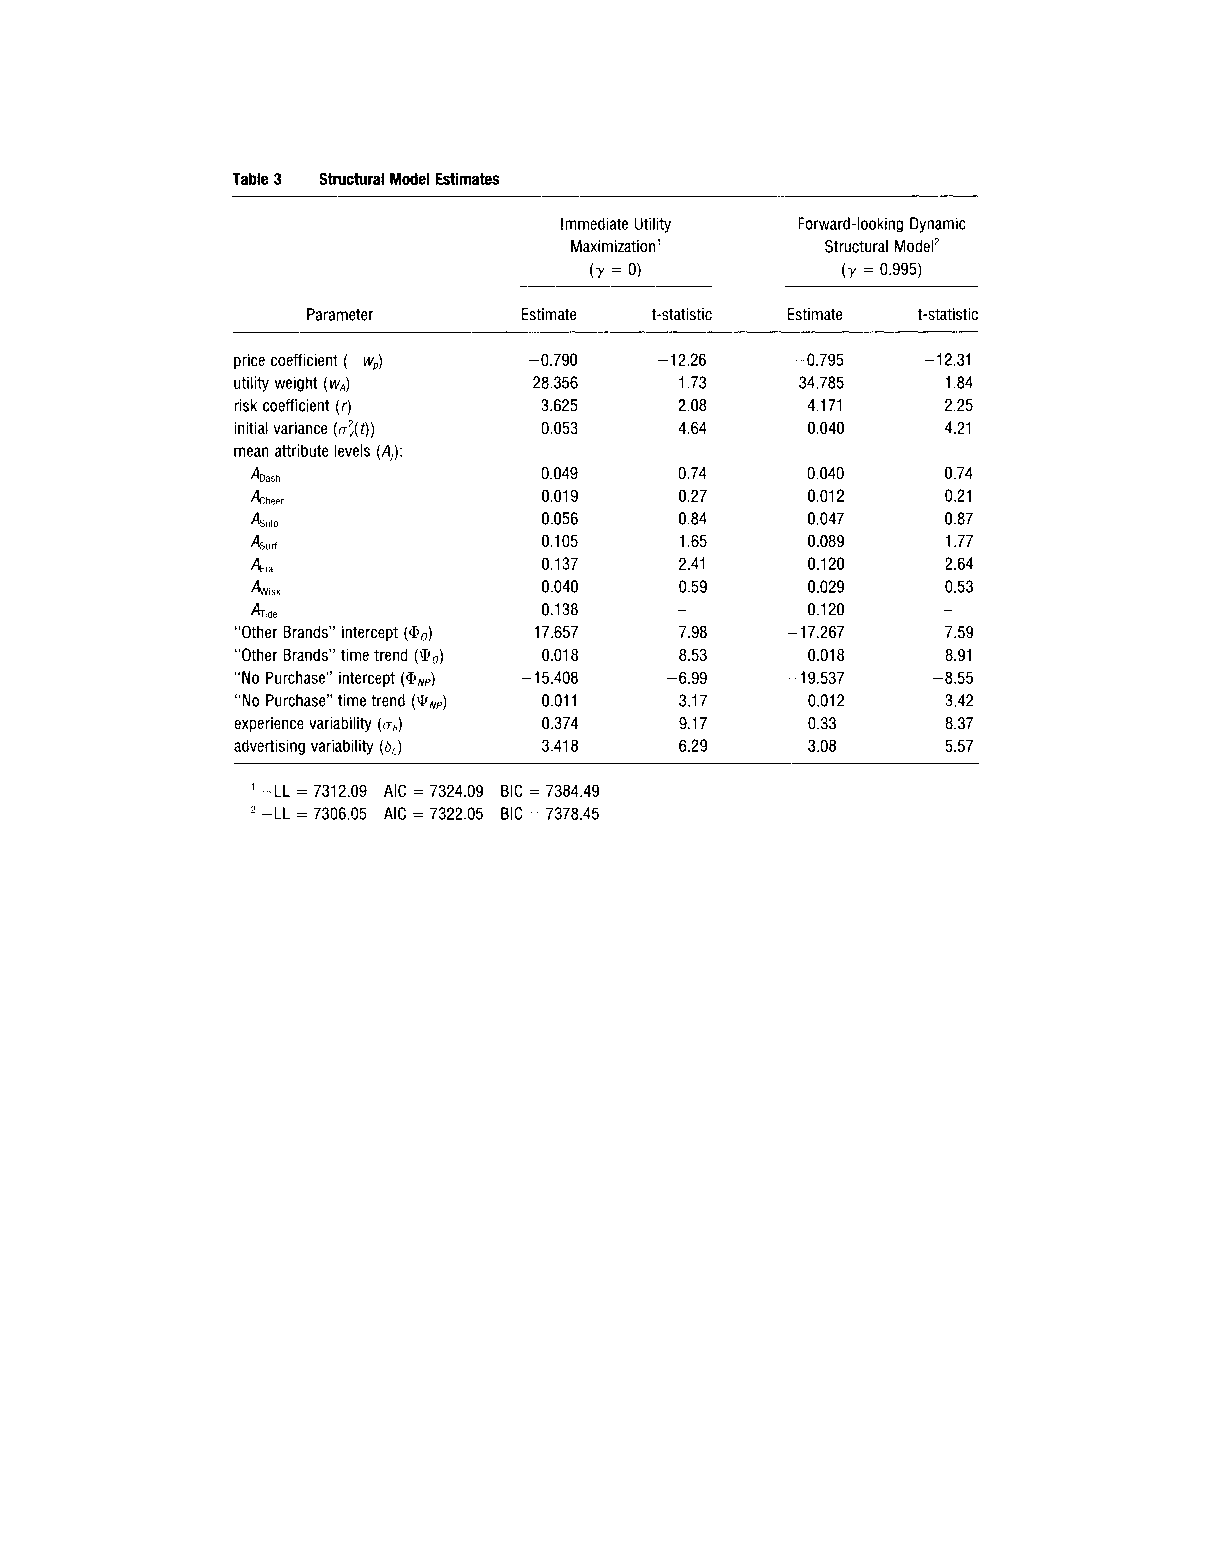
\includegraphics[width=4in]{resources/ek2.pdf}
\label{default}
\end{center}
\end{figure}
\end{frame}

\begin{frame}{Results}
\begin{itemize}
\item Static model has no effect of advertising (!)
\item Consumers are risk averse
\item Price coefficient negative and significant
\item Utility weight is huge (latent attribute -- cleaning power?)
\item Attribute levels are not significant (maybe differences are?)
\item Advertising more variable than experience
\item relatively small initial variance
\item Dynamic model shows \alert{more willingness to try new brands}
\end{itemize}
\end{frame}

\section*{Crawford and Shum}

\begin{frame}{Uncertainty and Learning in Pharmaceutical Demand}
Crawford and Shum (2005)
\begin{itemize}
\item  Italian anti-ulcer data: 34,972 patients (and a total of 98,634 prescription episodes)
\item Patients receive, on average, $2.8$ prescriptions for $1.2$ drugs over a period of just under 6 months.
\item Break up data into \textit{spells} or a sequence of one or more prescriptions of a single drug.
\begin{itemize}
\item A patient has 1.2 spells on average
\item An average spell is around 2.37 prescriptions
\end{itemize}
\item Probability of switching drugs is not constant over time
\begin{enumerate}
\item Early Switching: \alert{Experimentation} - about 10\% after first prescription
\item Late Switching: \alert{Learning} rise in switching at the end, especially for long-treatment length patients
\end{enumerate}
\end{itemize}
\end{frame}


\begin{frame}{Uncertainty and Learning in Pharmaceutical Demand}
\begin{figure}[htbp]
\begin{center}
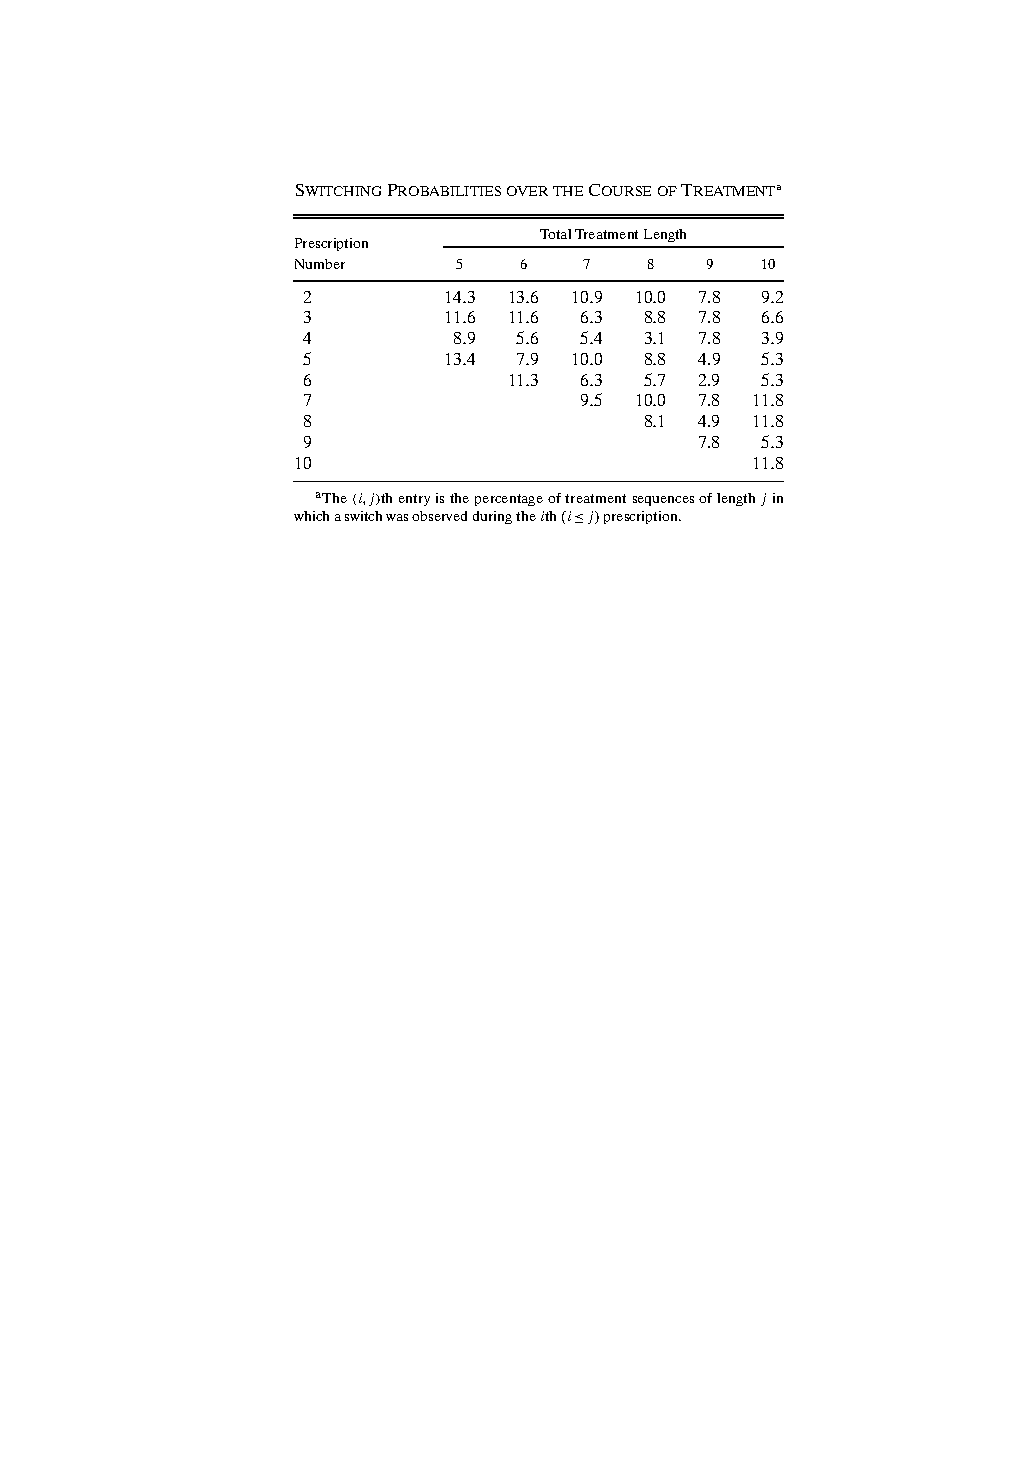
\includegraphics{resources/crawfordshum1.pdf}
\label{default}
\end{center}
\end{figure}
\end{frame}

\begin{frame}{Model Setup}
\begin{itemize}
\item Patients, $j$. Drugs, $n=5$, types $k=4$ (known to doctor-patient but not econometrician).
\item Treatment is characterized by two match values $(\mu_{jn},\nu_{jn})$ and two corresponding signals $(x_{jnt},y_{jnt})$ that correspond to the side-effects or curative probabilities respectively.
\item Patient's utility $u(\cdot)$ depends on side effects $x_{int}$
\item Cure probability $w(\cdot)$ depends on $y_{jnt}$
\item Don't know your match value  $(\mu_{jn},\nu_{jn})$  only the signal $(x_{jnt},y_{jnt})$, or treatment length $\tau = 1,\ldots,T$
\item Consumers have both signals $(x,y)$ and priors $(\mu,\nu)$ about side effects and cure probability
\begin{eqnarray*}
\left( \begin{smallmatrix} x_{jnt} \\ y_{jnt} \end{smallmatrix} \right)
&\sim& N \left( \begin{smallmatrix} \mu_{jn} \\ \nu_{jnt} \end{smallmatrix}, \begin{smallmatrix} \sigma^2_{jn} \\ \tau_{jnt}^2 \end{smallmatrix} \right) \\
\left( \begin{smallmatrix} \mu_{jn} \\ \nu_{jn} \end{smallmatrix} \right)
&\sim& N \left( \begin{smallmatrix} \overline{\mu}_{nk} \\ \overline{\nu}_{nk} \end{smallmatrix}, \begin{smallmatrix} \overline{\sigma}^2_{n} \\ \overline{\tau}_{n}^2 \end{smallmatrix} \right)
\end{eqnarray*}
\item Where $k=1,\ldots,4$ indexes the \alert{type specific priors}. 
\end{itemize}
\end{frame}

\begin{frame}{Model Setup}
\begin{itemize}
\item Doctors (without incentive problems) solve:
\begin{eqnarray*}
\max_{D=\{(d_{jnt})_{n=1}^N \}_{t=1}^{\infty}} E_D \sum_{t=1}^{\infty} \beta^t d_{jnt} u_{jnt}(1 - w_{j,t-1})
\end{eqnarray*}
\item Patients have CARA utility
\begin{eqnarray*}
u(x_{jnt},p_n,\epsilon_{jnt}) &=& -\exp(r *x_{jnt}) - \alpha p_n + \epsilon_{jnt}
\end{eqnarray*}
\item Derive the expected utility as:
\end{itemize}
\vspace{-0.5cm}
\begin{eqnarray*}
\tilde{EU}(\mu_{jn}(t),\nu_{jn}(t), p_n,\epsilon_{jnt}) &=& -\exp(r *\mu_{jn}(t) + \frac{1}{2} r^2(\sigma) (\sigma^2_n + V_{jn}(t))) \\
&& - \alpha p_n + \epsilon_{jnt}\\
&=& EU(\mu_{jn}(t),V_{jn}(t),p_n) + \epsilon_{jnt}
\end{eqnarray*}
\end{frame}

\begin{frame}{State Space}
\begin{itemize}
\item State Variables $S_t$:
\begin{itemize}
\item $(\mu_{jnt},\nu_{jnt}), I_{jnt}$ for $n=1,\ldots,5$ drugs.
\item $h_{j,t-1}$ (cure probability)
\item $\epsilon_{jnt}$
\end{itemize}
\item Recovery probability follows a Markov Process:
\begin{eqnarray*}
h_{jt}(h_{j,t-1},y_{jnt}) = \frac{ \left(\frac{h_{j,t-1}}{1-h_{j,t-1}} \right) + d_{jnt} y_{jnt}}  {1+ \left(\frac{h_{j,t-1}}{1-h_{j,t-1}} \right) + d_{jnt} y_{jnt}}  
\end{eqnarray*}
\item Beliefs follow Bayesian updating depending on $I_{jnt}$ the number of times patient $j$ takes drug $n$ at time $t$.
\end{itemize}
\end{frame}

\begin{frame}{Dynamic Decision Problem (DDP)}
Doctors face choice specific value function (infinite horizon, recovery state absorbing):
\begin{eqnarray*}
W(S_t) &=& \max_n [\exp(-r\mu_{jnt} + 0.5r^2(\sigma_n^2 + V_{jnt})) - \alpha p_n + \epsilon_{jnt}\\
&&+ \beta E[(1-h_{jt}(h_{j,t-1},y_{jnt}) E[W(S_{t+1}) | x_{jnt},y_{jnt},d_n=1] | S_t]\\
&=& \log [ \sum_n \exp[ \tilde{EU}(s) + \beta E[(1-h(s'))W(s') | d_n=1] | S_t] \\
&=& \max_n \{W_n(S_t)\}
\end{eqnarray*}
\end{frame}

\begin{frame}{Value Function}
\begin{eqnarray*}
W(S_t) &=& \max_n [\exp(-r\mu_{jnt} + 0.5r^2(\sigma_n^2 + V_{jnt})) - \alpha p_n + \epsilon_{jnt}\\
&&+ \beta E[(1-h_{jt}(h_{j,t-1},y_{jnt}) E[W(S_{t+1}) | x_{jnt},y_{jnt},d_n=1] | S_t]\\
&=& \log [ \sum_n \exp[ \tilde{EU}(s) + \beta E[(1-h(s'))W(s') | d_n=1] | S_t] \\
&=& \max_n \{W_n(S_t)\}
\end{eqnarray*}
\end{frame}

\begin{frame}{VFI + Simulate + Interpolate: (Keane Wolpin 1994): }
\begin{enumerate}
\item Define discrete grid $S^* \in S$
\item For each state $s \in S^*$ make an initial guess at the value function $W^0(s)$.
\item Run regression $W^0(s) = G(s)'\theta^0 + \varepsilon$
\item Draw the $M$ random signals $\{x_{jn}^m, y_{jn}^m\}$
\item Compute the expected value of choosing drug $n$ for each $s \in S^*S$, where $s^m$ is state corresponding to random draw $m$ and drug $n$ being chosen.
\begin{eqnarray*}
E[W(s | d_n =1,s)] = \frac{1}{M} \sum_m (1-h(s^m)) W^0(s^m)
\end{eqnarray*}
\item Update the value function for each $s \in S^{*}$
\item Iterate until convergence
\end{enumerate}
\end{frame}

\begin{frame}{Likelihood}
For $I_=0$ and $I_j=1$ censored and uncensored observations for patient $j$.
\begin{eqnarray*}
&&\sum_{k=1}^K p_k E_{\overline{x}_{jn T_{j}},k | h_{0,j,k}} \left[ \prod_{t=1}^{T_j-1} \left((1-h_{jt,k}) \prod_n \lambda_{jnt,k}^{d_{jnt}} \right) \right] \cdot h_{jT_j,k} \prod_n  \lambda_{jnt,k}^{d_{jnt}}\\
&&\sum_{k=1}^K p_k E_{\overline{x}_{jn T_{j}},k | h_{0,j,k}} \left[ \prod_{t=1}^{T_j-1} \left((1-h_{jt,k}) \prod_n \lambda_{jnt,k}^{d_{jnt}} \right) \right] \cdot \prod_n  \lambda_{jnt,k}^{d_{jnt}}\\
\end{eqnarray*}
($\lambda$ is logit choice probability)\\
We need to calculate expectations of joint distribution of $(\overline{x},h)$ by drawing $S=30$ sequences  per patient.
\end{frame}


\begin{frame}{Dynamic Model Parameters: Sick vs. Not so Sick}
\begin{figure}[htbp]
\begin{center}
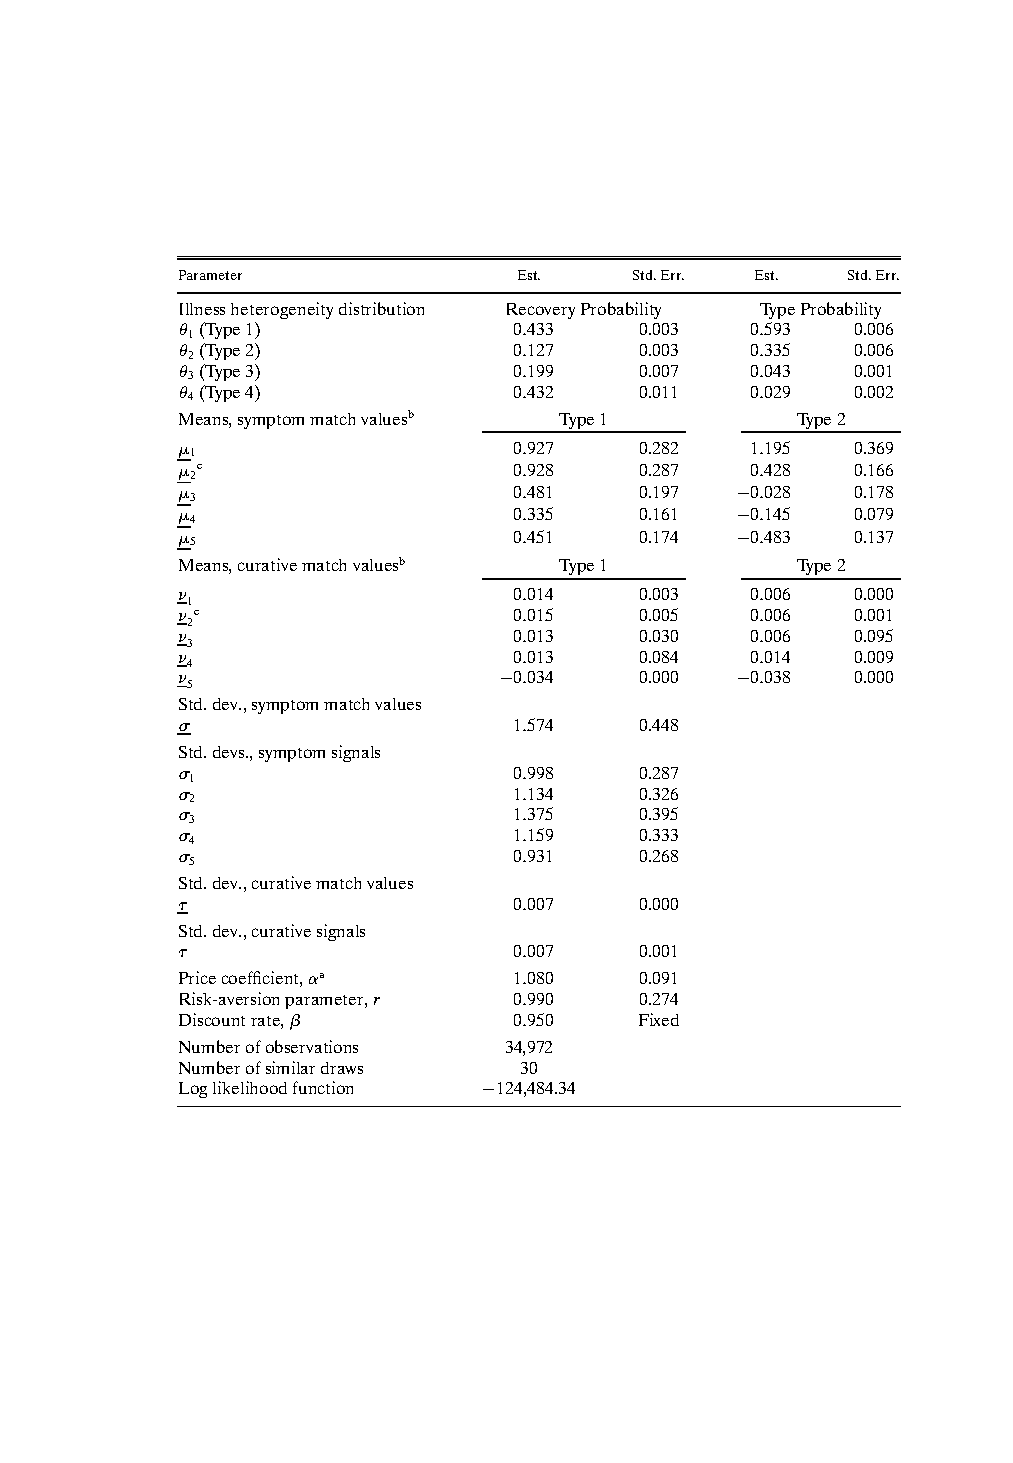
\includegraphics[width=7.5cm]{resources/crawfordshumparam.pdf}
\label{default}
\end{center}
\end{figure}
\end{frame}

\begin{frame}{Dynamic Model Parameters: Omeprazole (All types)}
\begin{figure}[htbp]
\begin{center}
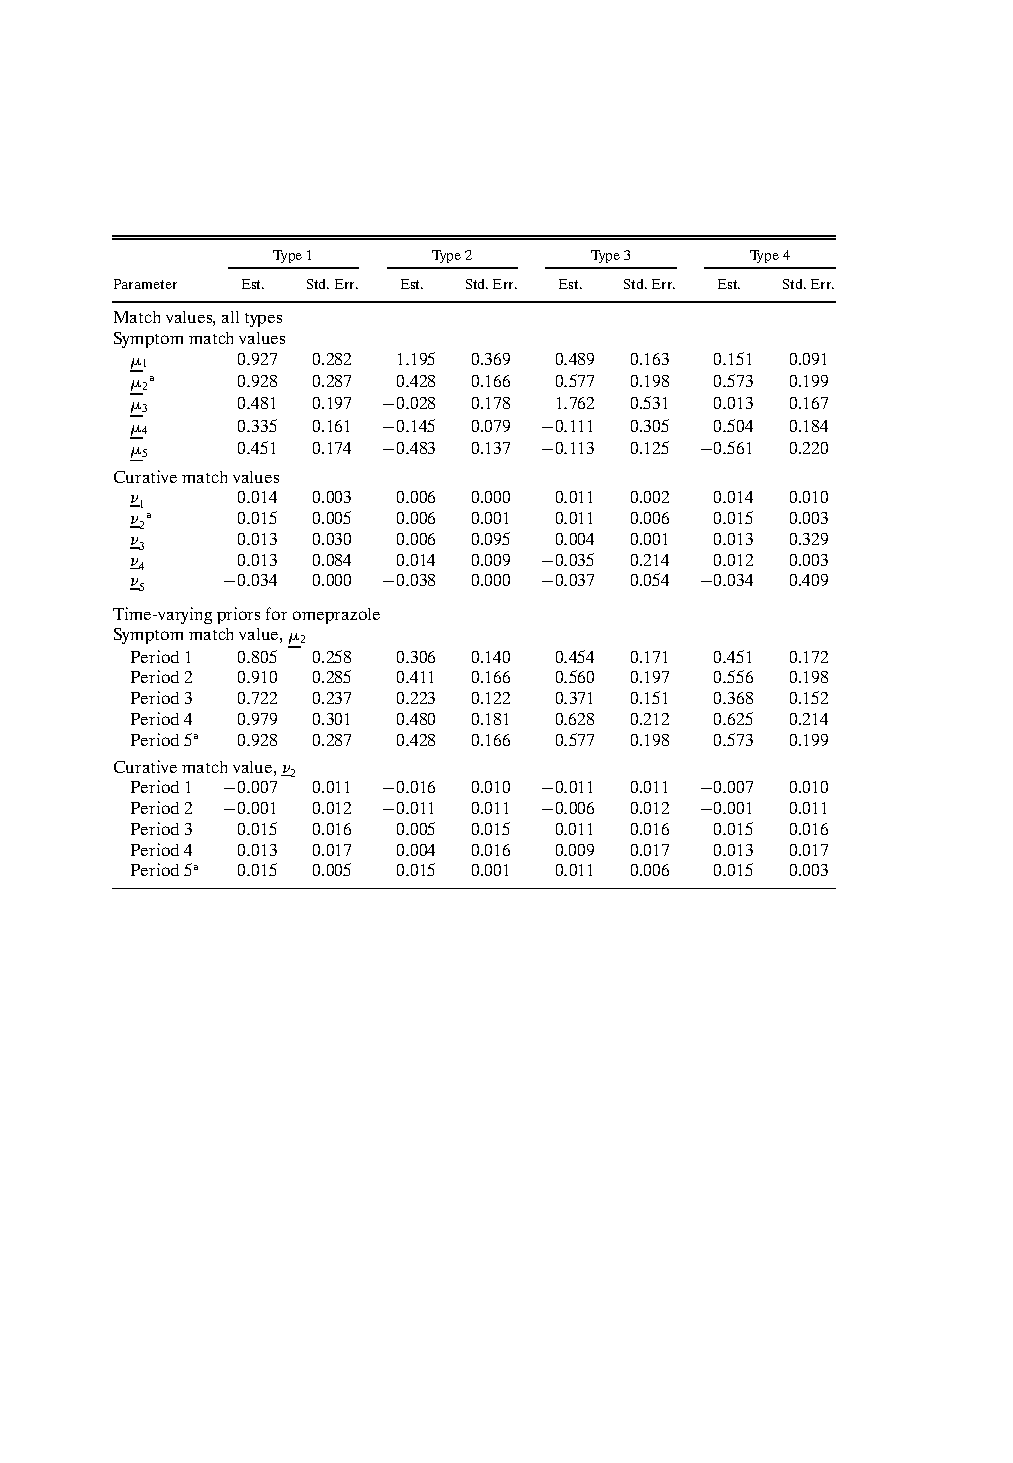
\includegraphics[width=7.5cm]{resources/crawfordshumparam2.pdf}
\label{default}
\end{center}
\end{figure}
\end{frame}

\begin{frame}{Results}
\begin{itemize}
\item Coefficient of risk aversion is high (switching costs?)
\item Learning happens very fast (variance falls from 2.48 to 0.7 after only \alert{one prescription}).
\item Learning slows after first prescription
\item Counterfactual (Complete Information): You know your match values which you draw from the same distribution but your perceived variance $V_{jn}^t = R_{jn}^=0$.
\begin{itemize}
\item Leads to more drugs $1.9$ instead of $1.4$.
\item Substitution away from market leader (no reason to stay with first drug). Lower HHI
\item Welfare up 9\%. Treatment up 80\%, cost up 60\%.
\end{itemize}
\item Counterfactual (Ban Experimenting): You are stuck with your first drug forever.
\begin{itemize}
\item Utility down 6\% but treatment length and costs about the same.
\item Wasn't much experimentation to begin with
\end{itemize}
\item Counterfactual (No Diagnostic Matching): Doctors can't learn types.
\begin{itemize}
\item Utility down 11\% and costs and length up 30-40\%.
\end{itemize}
\end{itemize}
\end{frame}

\end{document}













































